\chapter[Resample Like Sample]{Resample Like Sample: Blocked Resampling for Dependent Data} \label{ch4:resampling}
\chaptermark{Rethinking Resampling Methods}
\setlength{\epigraphwidth}{4.5in}
\epigraph{If two things are similar, the thought of one will tend to trigger the thought of the other.}{Aristotle, \textit{``Laws of Association''}, 300 B.C.}

%----------------------------------------------------------------------------------------------------------------------------------------------------------------------------------------------------------
\section*{Summary}
Having chosen and fitted an estimator based on observations, we need to answer further questions about the accuracy of the estimator or the likely quality of inferences. Most resampling techniques used in water resources modeling employ a simple nonparametric random splitting of data into a number of folds to estimate model error (i.e., k-fold cross-validation). In each iteration, one fold is held out as a test set and others are designated as a training set. While suitable for independent and identically distributed (iid) random variables, such random resampling schemes can ignore structures in dependent data, and underestimate model error. The central assumption here is that training and evaluation data are independent. If not, error estimates will be too optimistic, and model selection will favor more complex models \cite{roberts2017cross}. % Also, models evaluated with randomized cross-validation methods disregard the assumption of independence of residuals. When mapping the residuals in time or in space, the trends point to dependence structures in the data that produce an over-fit model with non-causal parameters or missed meaningful parameters. %cite?

For the PUB problem, more accurate estimates of model error can come from techniques that block training sets in time, space, or unique structure (e.g., by hydrologic basin networks). Blocked methods give us a collection of ``approximately independent'' and ``identically distributed'' random vectors. The difficulty here lies in specifying block sizes and structures. Blocking potentially reduces the range of parameters seen by the model, or may exclude a particular meaningful combination of predictor variables in the training data set. Too small of a block size and the resampling strategy more closely mimics the randomized method and runs the risk of under estimating model error. Large block sizes force too much model extrapolation and risk over estimating model errors. 

This chapter compares the following random and blocked resampling methods: resubstitution (i.e., training set is test set), random k fold  (or Monte Carlo), leave one group out (LOGO), and leave multiple groups out (LMGO) cross-validation strategies as well as, random or independent and identically distributed (IID), blocked by group (BBG), and blocked by multiple groups (BBMG) bootstrapping strategies. Of the four model types (i.e., LM, GLM, RF, and NN discussed in chapter \ref{ch2:transformations}), the LM performs the poorest and is also least sensitive to the resampling scheme (bR\textsuperscript{2} ranges from 0.23 to 0.26). The RF is most sensitive to the resampling scheme; larger the block sizes perform worse (bR\textsuperscript{2} is 0.51 for LMGO, largest block size, and 0.94 for resubstitution, no blocking). Surprisingly, in the NN, the more \textit{appropriate} the block size the better it performs (bR\textsuperscript{2} is 0.75 for randomized 2 fold, which has a large fold size but not blocked systematically, and 0.92 for LOGO, which blocks by basin that is the natural grouping scheme). In the NN, even the LMGO method out-performs the randomized k fold methods proving that in the NN intelligent blocking (i.e. by basins) proves more useful even though the block size is large (i.e., multiple basins in a block rather than just one). 

As expected, when using bootstrapped resampling, models built with the IID method appear to perform better on average and are more reliable (have smaller spread). However, IID resampling underestimates model error and overestimates its reliability, so, true model error is closer to those of the BBG and BBMG methods. Generally, regardless of model type, larger block sizes produce more uncertain model results (i.e., more spread in BBMG and BBG than in IID estimates). These results illustrate the sensitivity of each model's estimated uncertainty to resampling methods, and its importance in designing a resampling strategy. 
% leave hierarchies out (LHO) and blocked by hierarchy (BBH) deleted cause we didn't perform these experiments.

%----------------------------------------------------------------------------------------------------------------------------------------------------------------------------------------------------------
\section{Introduction} \label{ch5:introduction}
Having chosen and fitted an estimator $\hat{\theta_n}$ based on observations, $X_n$, we need to evaluate the accuracy of the estimator $\hat{\theta_n}$ and the quality of inferences made based on $\hat{\theta_n}$. Bootstrap and other resampling methods are general methods for finding estimators of parameters like MSE($\hat{\theta_n}$). In predictive modeling, the estimator needs to be accurate at unmeasured locations: either ungauged locations, or at future times where observations do not yet exist. Therefore, the predictive accuracy of the \textit{training set}, the data the model is trained on, is of little consequence. The \textit{test set} error, the error of a set of data not seen by the model, is a better measure of model accuracy. 

Test set error can be easily calculated if such a data set exists, or, it can be estimated by holding out a subset of the training data. The holding-out is done by resampling strategies, to create an otherwise non-existent test set. Two popular resampling methods are: \textit{cross-validation} and \textit{bootstrapping}. In cross-validation, the data set is split into non-overlapping testing and training data sets where each observational unit gets a chance at being in the test set once. In bootstrapping, sampling is done with replacement where each observational unit has an equal chance at being selected and being selected more than once. In this case, the probability that the observation $X_0 = x_i$ appears in the training sample is $1- (1 - 1/n)^n \approx 0.632$ \cite{efron1997improvements}. Therefore, in bootstrapping, approximately 1/3\textsuperscript{rd} of the data set will end up not being selected and are ``out-of-bag'' from training. 

Resampling helps avoid problems caused by an unknown ``population''; if the resampling method is chosen appropriately then, the ``resample'', together with the sample, is expected to reflect the original relation between the population and the sample \cite{lahiri2013resampling}. Appropriate resampling is one where the same dependence structures seen in the sample appear in the resample. The goal is to approximate the data generating mechanism as well as possible or ``resample like the sample.'' 

Geographic data often have internal correlation and dependence structures \cite{legendre1993spatial}: (1) temporal autocorrelation: nature responds to changes gradually. For example, today's precipitation is correlated with yesterday's precipitation; (2) spatial autocorrelation: nearby things tend to be more related than those far away. For example, two points close together on a topographic map are more likely to have similar elevations;  and (3) hierarchical structures: the network of streams flowing into one another (or more formally, the stream order) provides a hierarchical structure. That is, basin topology provides a spatial structure more complicated than mere proximity of river gauges. For example, two points on a river may be close in proximity but depending on which side of the watershed divide they fall on they can be fed by two different basins, in different hierarchies in the network, with different governing hydrologic processes and so, have different measured flows (Figure \ref{fig:structured}). 

\begin{figure}[ht]
	\centering
	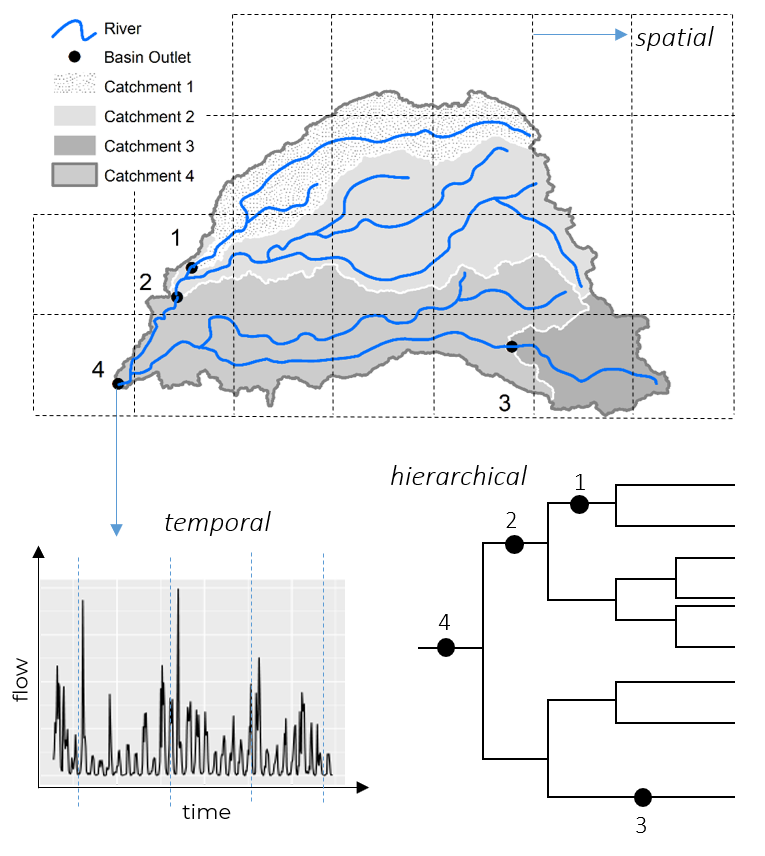
\includegraphics[width=12cm,trim={0 0 0 0},clip=true]{plots/ch4_structured.png}
	\caption[Dependence structures in streamflow data.]{Dependence structures in streamflow data are: temporal autocorrelation, spatial autocorrelation, and hierarchical structures.  Appropriate resampling is one where the same dependence structures seen in the sample appear in the resample.} 
	\label{fig:structured}
\end{figure}

A dependence structure points to a pseudo replication problem (Figure \ref{fig:marbles}). For an observation, $x^d$, at a distance, $\Delta d$, from another observation, $x^{d+\Delta d}$, where $x^d$ and $x^{d+\Delta d}$ are autocorrelated, the distance $\Delta d$ can be defined in time, space, or hierarchy. In random resampling, either autocorrelated value is free to lie in the bag of samples given to the model, or be left out-of-bag. Therefore, the model can easily predict one, given that the other is likely in the bag. However, in blocking resampling the two observations are connected and will both end up in the bag or out-of-bag. Here, the model is forced to predict a phenomenon from other observations. 

\begin{figure}[ht]
	\centering
	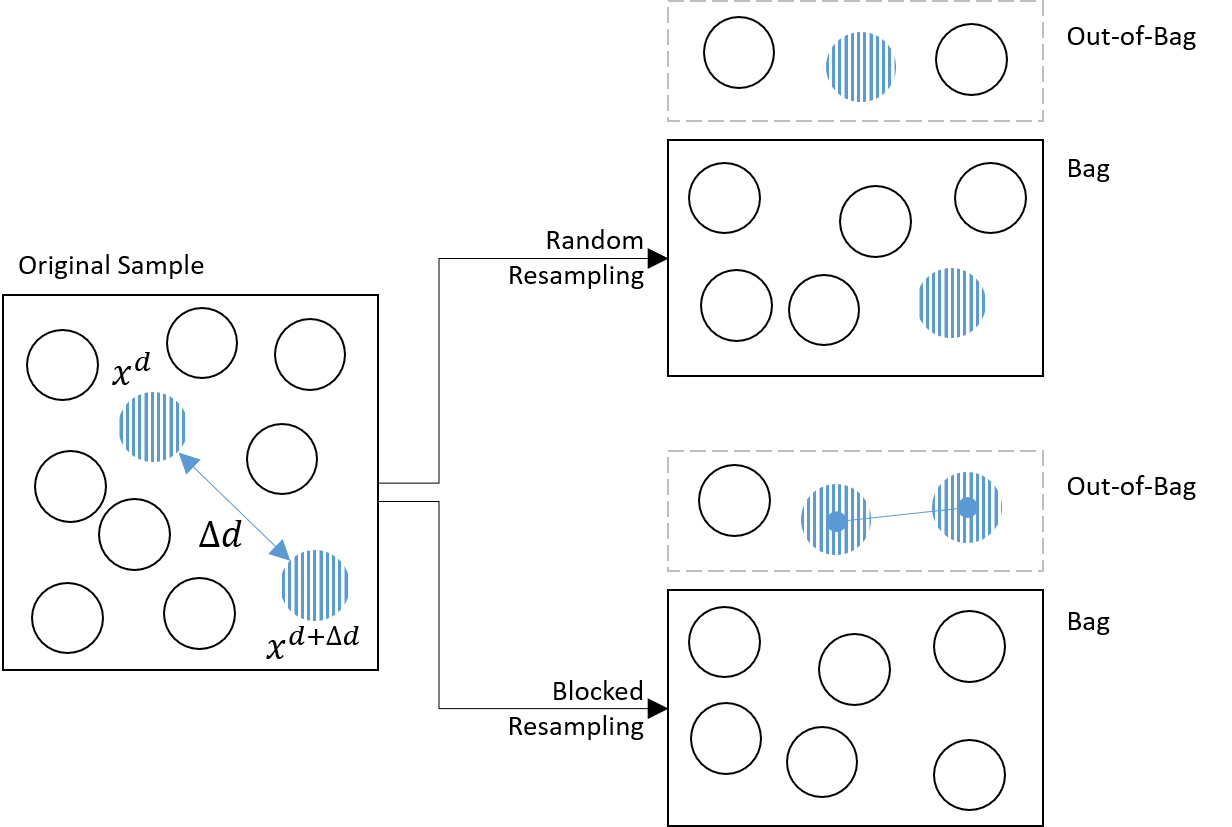
\includegraphics[width=10cm,trim={0 0 0 0},clip=true]{plots/ch4_resampling.png}
	\caption[Autocorrelation as a pseudo replication problem.]{Autocorrelation as a pseudo replication problem. The two striped marbles are autocorrelated. A model that uses random resampling will be able to easily predict one striped marble since it has seen the other. When blocking, the observations move in and out of the bag together.} 
	\label{fig:marbles}
\end{figure}

Most studies in water resources ignore dependence structures in the data when devising a resampling strategy. When test data are randomly selected from the entire temporal, spatial, and hierarchical domain, training and testing data from nearby locations will be dependent due to \textit{autocorrelation}. Therefore, if the objective is to project outside the spatial structure of the training data (e.g., to an ungauged basin), error estimates from random resampling, will be overly optimistic. This chapter will compare a model's error estimates given multiple random and blocking resampling strategies. 

Moreover, cross-validation has been the traditional method used for the predictive accuracy problem and provides a nearly unbiased estimate of the future error rate. However, the low bias of cross-validation is often paid for by high variability. \citeA{efron1997improvements} showed that suitably defined bootstrap procedures can substantially reduce the variability of error rate predictions. Bootstrapping and its blocked variants are now the preferred method for resampling in statistics, while cross-validation still remains popular in water resources. This chapter applied both methods to PUB models. 

% Why bother? 
% While correlation structures may not be as problematic in conventional statistics, combined with high-dimensions and low sample sizes, predictive methods suffer. Compounding the problem can be low computational abilities (Figure \ref{fig:blocksizes}).
%
%\begin{figure}
%	\centering
%	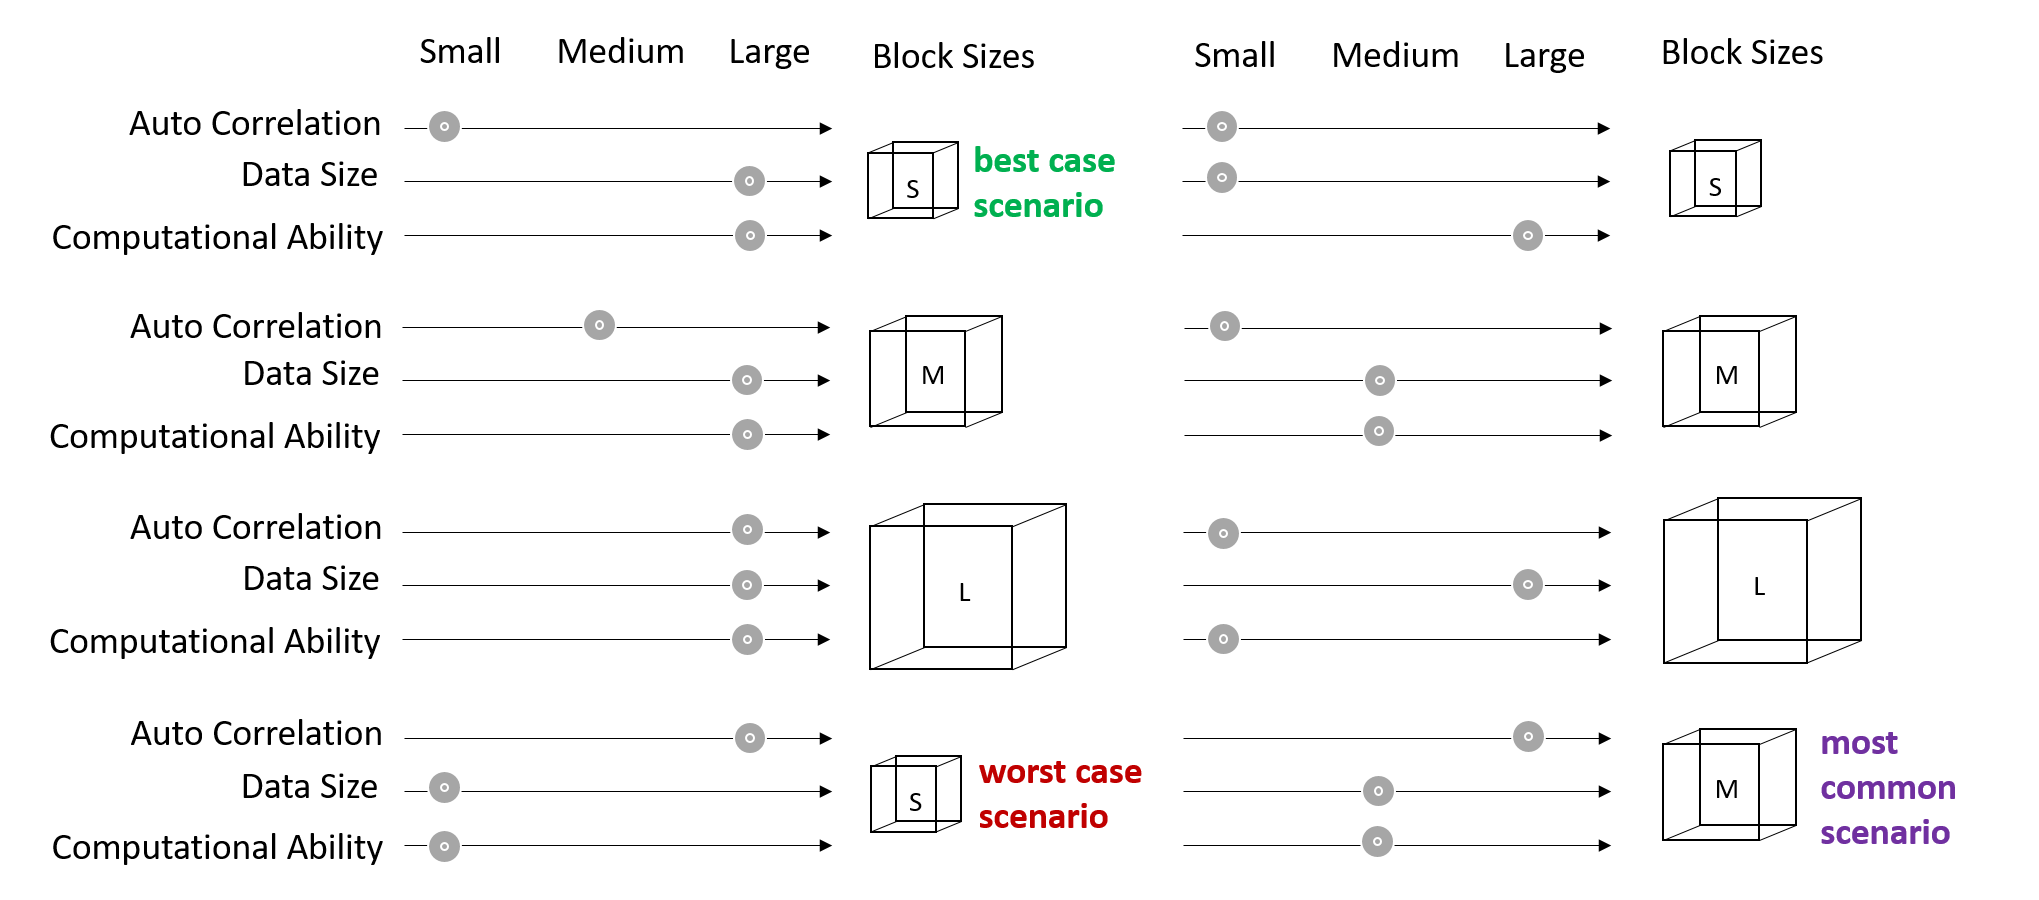
\includegraphics[width=15cm,trim={0 0 0 0},clip=true]{plots/blocksizes.png}
%	\caption{The block size in resampling methods is a function of the autocorrelation, data size, and computational ability.} 
%	\label{fig:blocksizes}
%\end{figure}

% Moreover, the predictive accuracy of the model on the training set can severely differ from the test set. With increasing model complexity (e.g., adding parameters to the model), clearly the model will fit the training data increasingly well. However, errors in the test set behave differently as is evident in the characteristic U-shape of the bias-variance tradeoff curve \cite{friedman2001elements}. The expected error in the test set is a polynomial of power two (Equation \ref{eq:bvt}) and is comprised of variance, bias, and a constant term. In the first portion of the U, bias will decrease more than the gain in variance, however, past some point, we are now overfitting and the gain in variance is too much to be offset by the decrease in bias. Therefore, depending on how we specify the model, we will lie somewhere along this U shape and cannot substitute training error rates for the true predictive capability of the model. 

% Resampling methods are generally used to either: (1) estimate the accuracy of sample statistics (e.g., the standard deviation of an $\alpha$ parameter in a linear model $y=\alpha x+\beta$); (2) estimate the accuracy of significance tests (e.g., p-values); or (3) test the models. In hydrology, when examining observed data, the true population (i.e., the set of all possible hydrologic states) is unknown and the true error in the model or a sample statistic is unknowable. Therefore, we commonly use resampling methods to test our model's predictions. 

% With the test set, that is held out observed data, and our model's results, we can conveniently apply any statistical measure of fit desired as a proxy for model accuracy (e.g., Nash-Sutcliffe Efficiency (NSE)). 

%-----------------------------------------------------------------------------------------------------------------------------------------------------------------------------------------------------
\section{Methods}
To find the test set error of the estimator we: (1) simulated $n$ landscapes of the data by resampling the original data set using a chosen resampling method. This separates the data into training and testing sets; (2) for each simulation, fed the training data into the desired machine learning algorithm (i.e., LM, GLM, RF, and NN); and (3) calculated the desired model measure of fit for each simulation (Figures \ref{fig:cvmethods} and \ref{fig:bsmethods}).

% (4) compare the Probability Density Function's (PDFs) of the model measures of fit with that of an ``ideal'' or appropriately resampled data.   

\begin{figure}[ht]
	\centering
	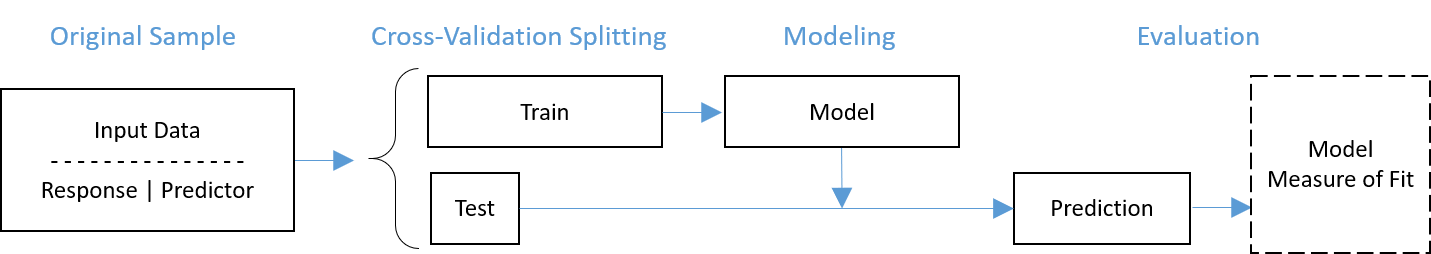
\includegraphics[width=15cm,trim={0 0 0 0},clip=true]{plots/ch4_cv_flowchart.png}
	\caption[Cross-validation research design.]{Research design for cross-validation resampling to estimate model error.} 
	\label{fig:cvmethods}
\end{figure}

\begin{figure}[ht]s
	\centering
	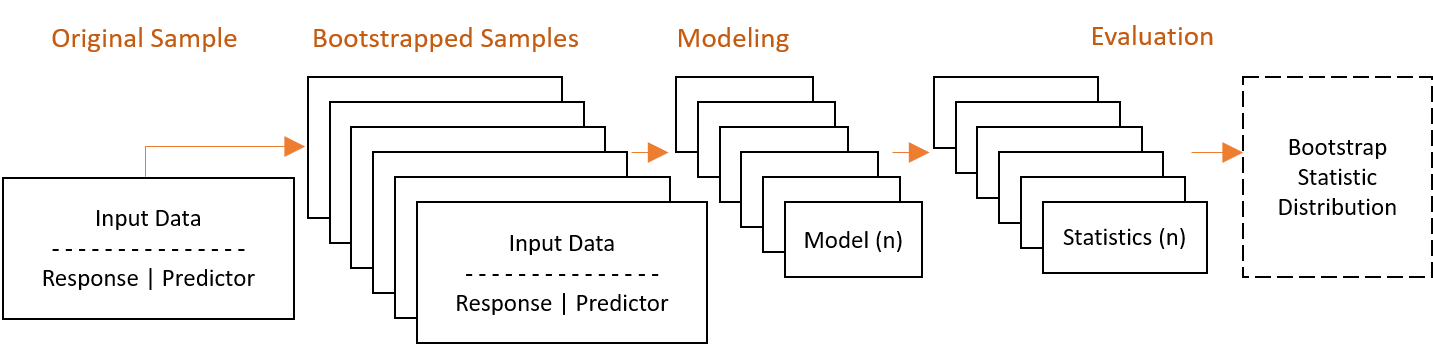
\includegraphics[width=15cm,trim={0 0 0 0},clip=true]{plots/ch4_bs_flowchart.png}
	\caption[Bootstrapping research design.]{Research design for bootstrapped resampling to estimate the distribution of the bootstrap statistic.} 
	\label{fig:bsmethods}
\end{figure}

Separating the data into training and testing sets (step 1), can be done by one of the following methods: 

\textbf{Cross-Validation}
\begin{itemize}
	\item Resubstitution: The test set is the training set. Here, the model is evaluated against the same data it has already seen. We expect the model to perform the best here with the distribution of residuals closest to zero. 
	\item Randomized k fold or Monte-Carlo:
		\subitem Two fold or validation set: The test set is a random 1/2 of the full data set. The training set is the other 1/2. This method is run twice, once with the first half as a test set and next with the second half as the test set. 
		\subitem Five fold: The data is split into five folds. In each iteration each fold is considered the test set and the other four folds the training set. 
		\subitem Ten fold: The data is split into ten folds. In each iteration each fold is considered the test set and the other nine folds the training set. 
	\item Leave One Out (LOO): In each iteration, one instance of the data is held out, and the rest of the data set is the training set. This method was too computationally intense to perform on our data set.
	\item Leave One Group Out (LOGO): In each iteration, one basin's data is held out as a whole and the rest of the basins become the training set. The process is repeated for each basin. 
	\item Leave Multiple Groups Out (LMGO): In each iteration, 1/5\textsuperscript{th} of the basins are held out and the other basins become the training set. The process is repeated for each fold. 
	\item Leave Hierarchies Out (LHO): Blocking is designed across basins that cluster on a river branch. Because of the limited size of the dataset we have not considered this strategy. 
\end{itemize}

\textbf{Bootstrapping}
\begin{itemize}
	\item Randomized or IID: It is the most popular form of bootstrapping where a new data set is built from randomly resampling the original sample with substitution. The length of the data set is the original length of the data set.
	\item Blocked By Group (BBG): the data set is blocked by unique basins. The basins are randomly resampled with substitution. Since the basins may have differing record lengths, the length of the data set may not match the original data set. However, the data set will have the same number of basins as in the original data set. 
	\item Blocked By Multiple Groups (BBMG): The data set is blocked by multiple basins. The grouped basins are randomly resampled with substitution. As the group sizes become larger the blocking size becomes larger. 
	\item Blocked By Hierarchy (BBH): Blocking is designed across basins that cluster on a river branch. The grouped basins are randomly resampled with substitution. Because of the limited size of the dataset we have not considered this strategy.
\end{itemize}

The most appropriate resampling method is those which block observations in groups. In LOGO cross-validation or BBG bootstrapping the correlation structure is simplified; we make the assumption that data are correlated within a basin, but independent between basins. The structure of the block bootstrap is easily obtained (where the block just corresponds to the group), and only the groups are resampled, while the observations within the groups are left unchanged \cite{cameron2008bootstrap}.

% NOT RELEVANT HERE, MAKE A NEW CHAPTER MAYBE?
% Most studies, also fail to examine the autocorrelation of the errors produced by the developed models; as such, inferential results can be biased. Either including additional predictor variables, or choosing a different functional form has to be considered if a strong autocorrelation is detected in the model's residuals. The problem of inference cannot be diagnosed without explicitly checking for the spatial and temporal variability of the residuals, which are supposed to be independent and not correlated. A simple visual check or a formal test of the significance of Moran's I or Geary's C can help in this regard. 

% In this study, data from a mechanistic simulation model, the Basin Characterization Model (BCM), with fitted values are considered as ``true'' unimpaired flows. The BCM approximates California hydrology well. It estimates monthly unimpaired flows and is developed and maintained by the U.S. Geological Survey (USGS). The data spans California at 270m x 270m resolution. The recharge and runoff estimates from the BCM are attained from physically based equations that calculate potential evapotranspiration, snow, excess water, and actual evapotranspiration. Depending on soil properties and the permeability of underlying bedrock, surface water can be classified for each cell as either recharge or runoff \cite{flint2014california}. 

% In both the cross-validation and bootstrap, the resampling results are compared to an ``ideal'' MSE, which was calculated by: (1) producing one model for each simulated landscape; (2) using said model to predict to the other $n-1$ landscapes; (3) using the predicted and observed values to calculate the MSE for each $n-1$ landscape; (4) averaging the MSE of the $n-1$ landscapes; (5) repeating the process for all $n$ landscapes; and (6) resulting in $n$ MSEs, one for each landscape, which can be plotted as a PDF (Figure \ref{fig:idealmethod}). 

% can use a parametric bootstrap, but explain the high dimensionality of the problem

%\begin{figure}[ht]
%	\centering
%	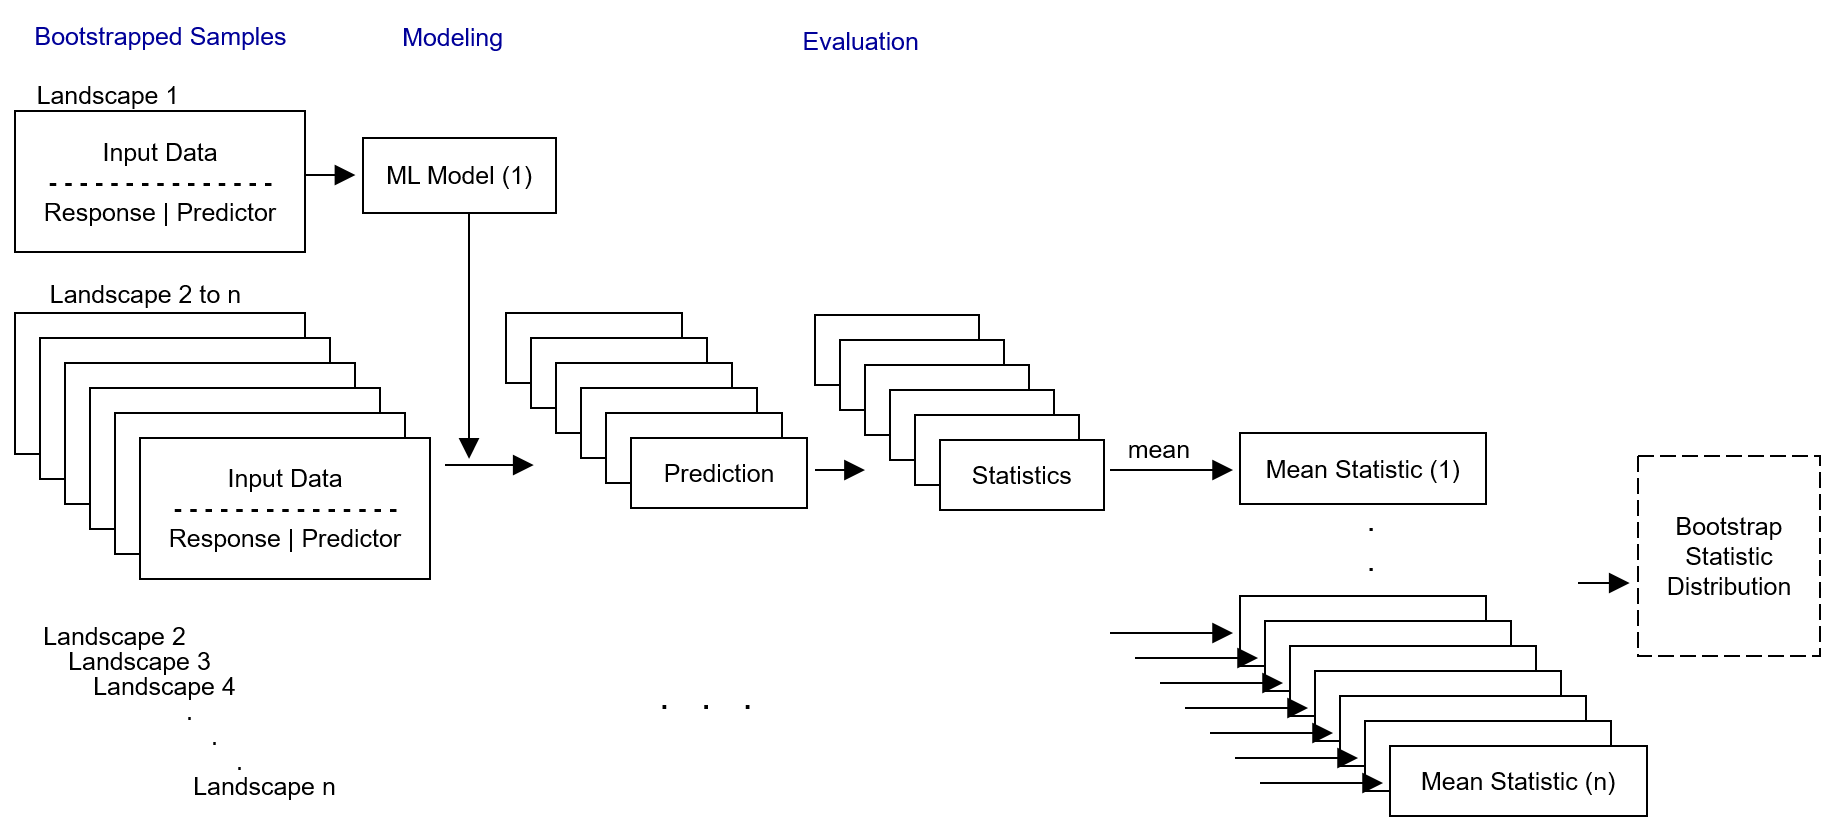
\includegraphics[width=15cm,trim={0 0 0 0},clip=true]{plots/ideal_flowchart.png}
%	\caption{Research design: compare the errors with that of an ``ideal'' model.} 
%	\label{fig:idealmethod}
%\end{figure}

%-----------------------------------------------------------------------------------------------------------------------------------------------------------------------------------------------------
\section{Results}

%-----------------------------------------------
\subsection{Model Evaluation}

Figure \ref{fig:cvbserrors} shows that generally, in the LM, GLM, and RF, the test set error is lower for smaller block/fold sizes. The LOGO and BBG methods provide the most accurate estimates, since they replicate the natural grouping by basin of the sample in the resample. Therefore, in PUB modeling with an RF, a ten fold cross-validation strategy can underestimate model error (bR\textsuperscript{2}=0.79 in random ten fold vs. 0.61 in LOGO). The same is true in bootstrapping;  IID bootstrapping underestimates model error (bR\textsuperscript{2}=0.79 vs. 0.50 in BBG). Surprisingly, the NN performs better given a more accurate cross-validation technique (LOGO bR\textsuperscript{2}=0.92). In bootstrapping, the IID suffers the same fate as in other models and gives artificially low estimates compared to the BBG and BBMG methods. Overall, the performance in each method is clustered together with the NN and RF performing very similarly with the different cross-validations strategies. 

\begin{figure}
	\centering
	\begin{subfigure}{\textwidth}
  		\centering
 		 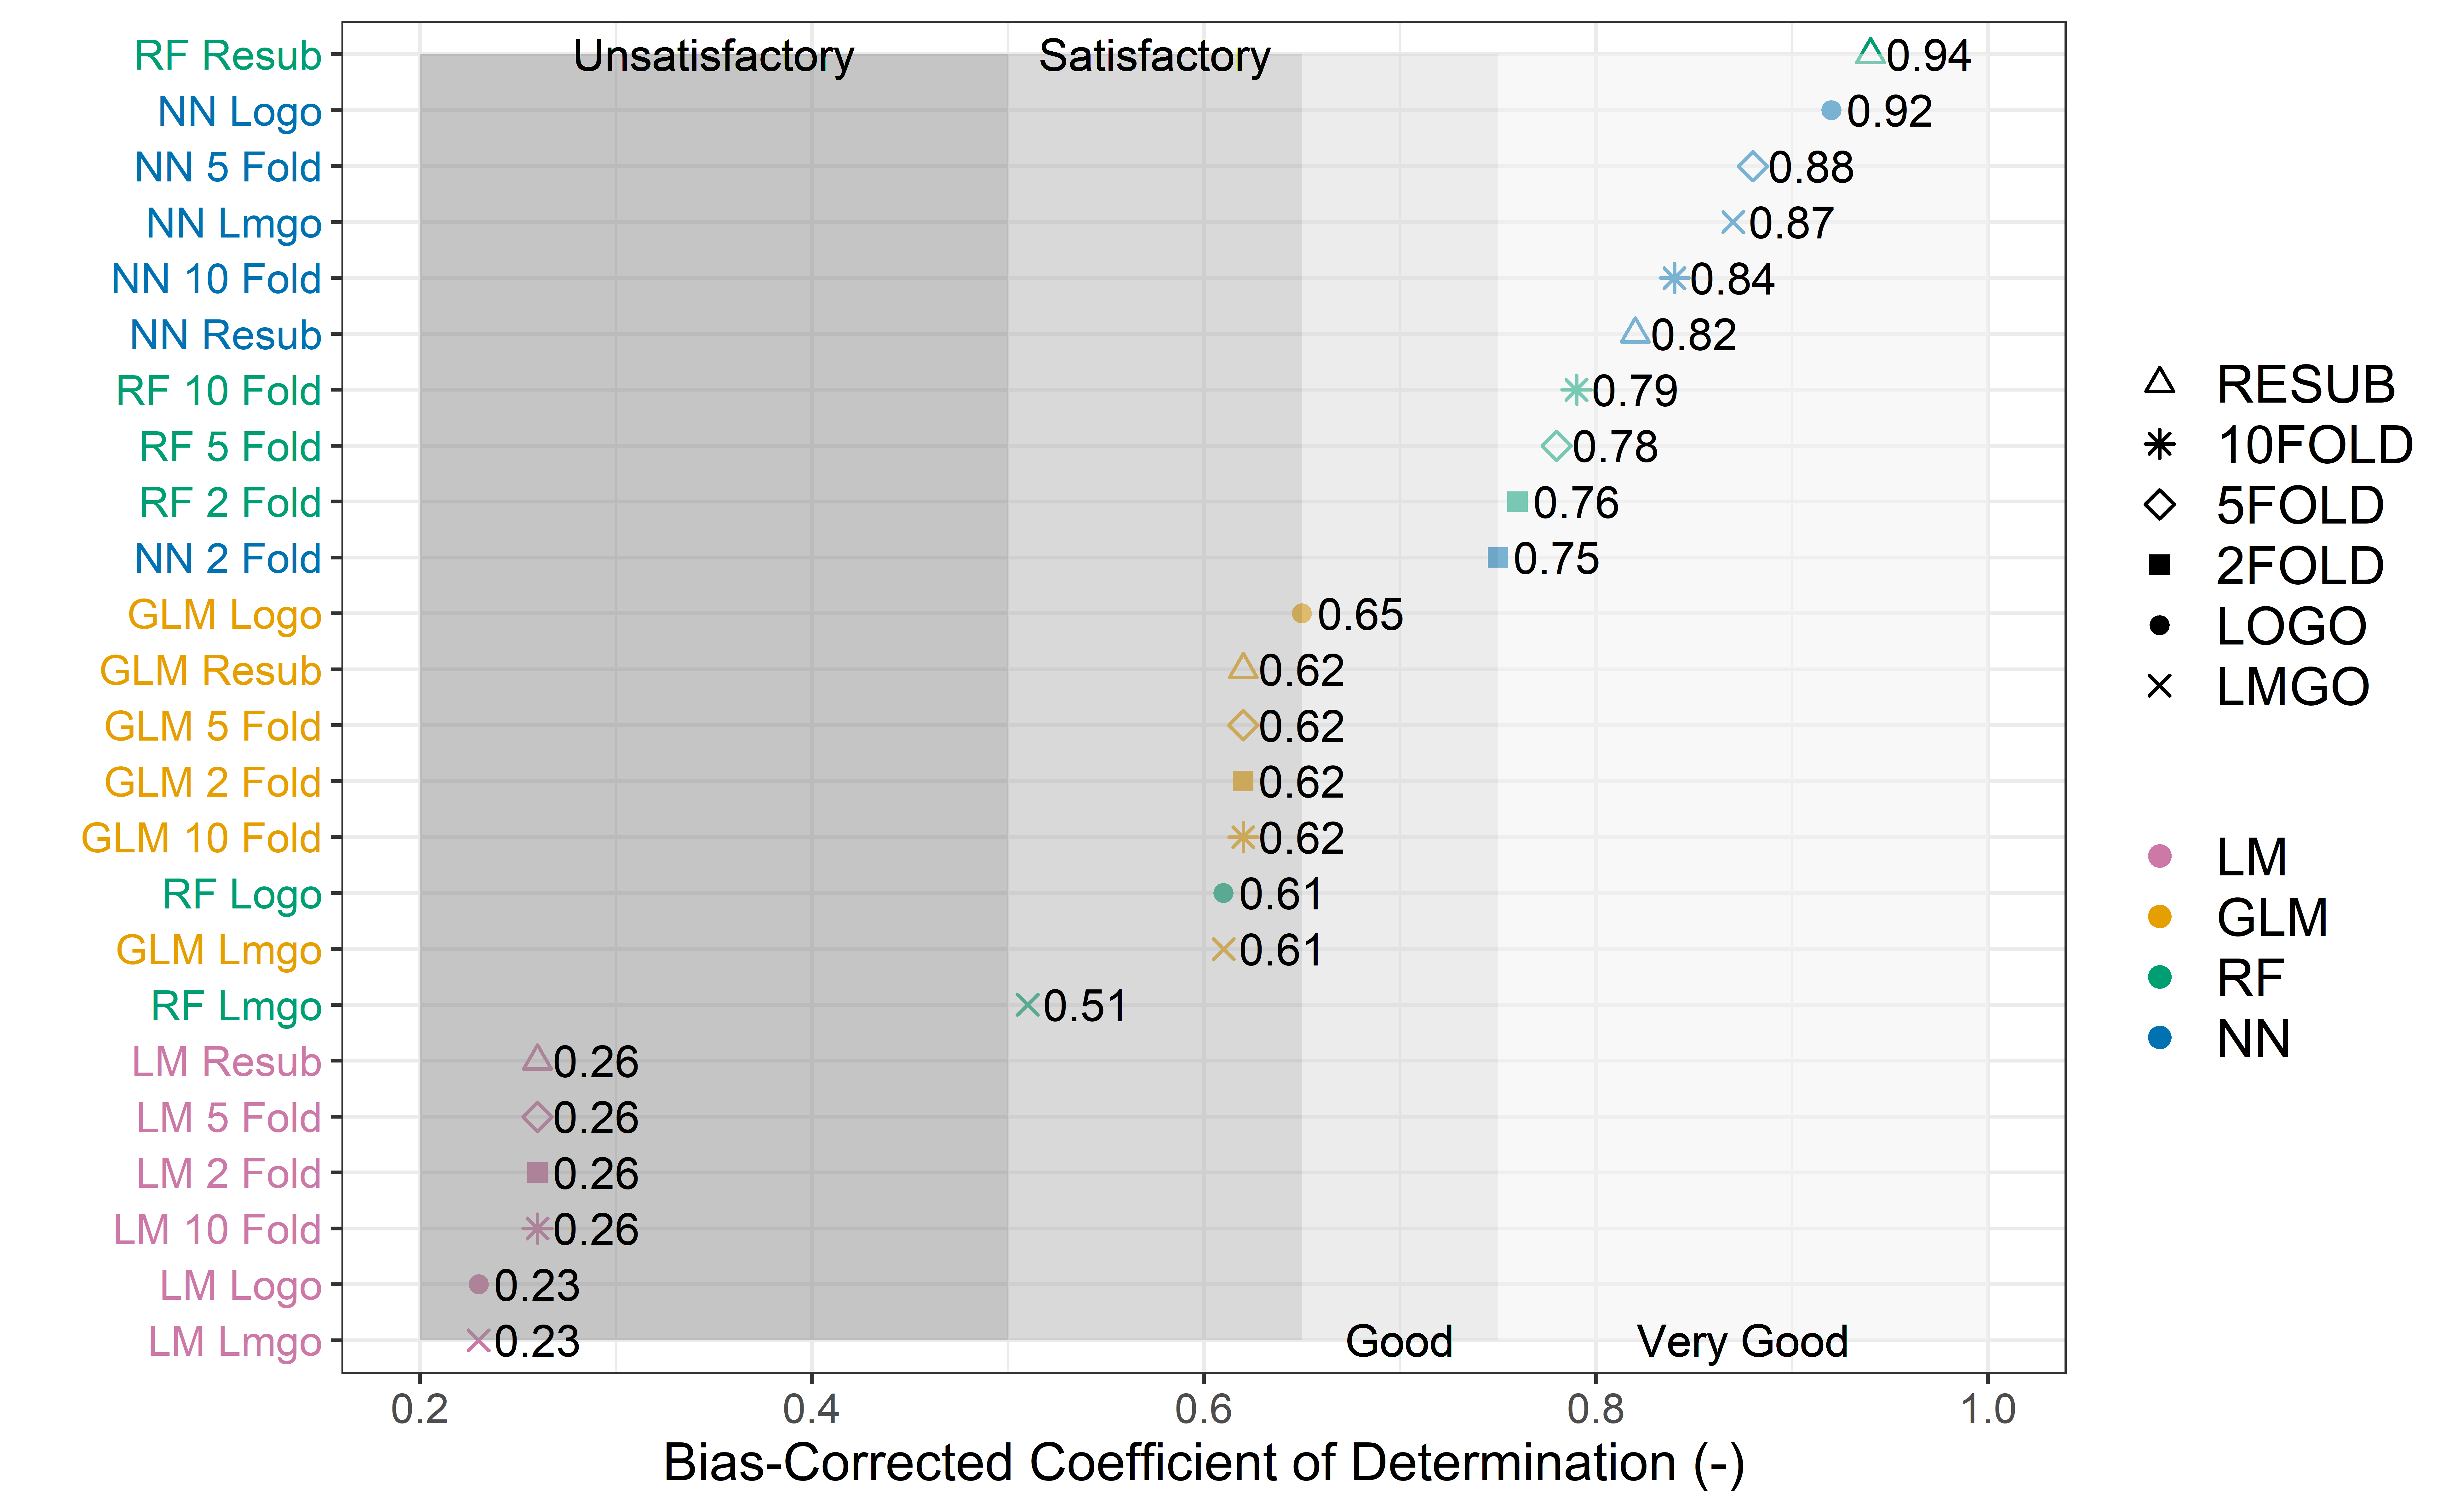
\includegraphics[width=\textwidth, trim={0 0 0 0}, clip=true]{plots/rplot41_gof_bR2.png}
  		\caption{The cross-validation test set error.}
  		\label{fig:cvmoderror}
	\end{subfigure} 
	\begin{subfigure}{\textwidth}
  		\centering
  		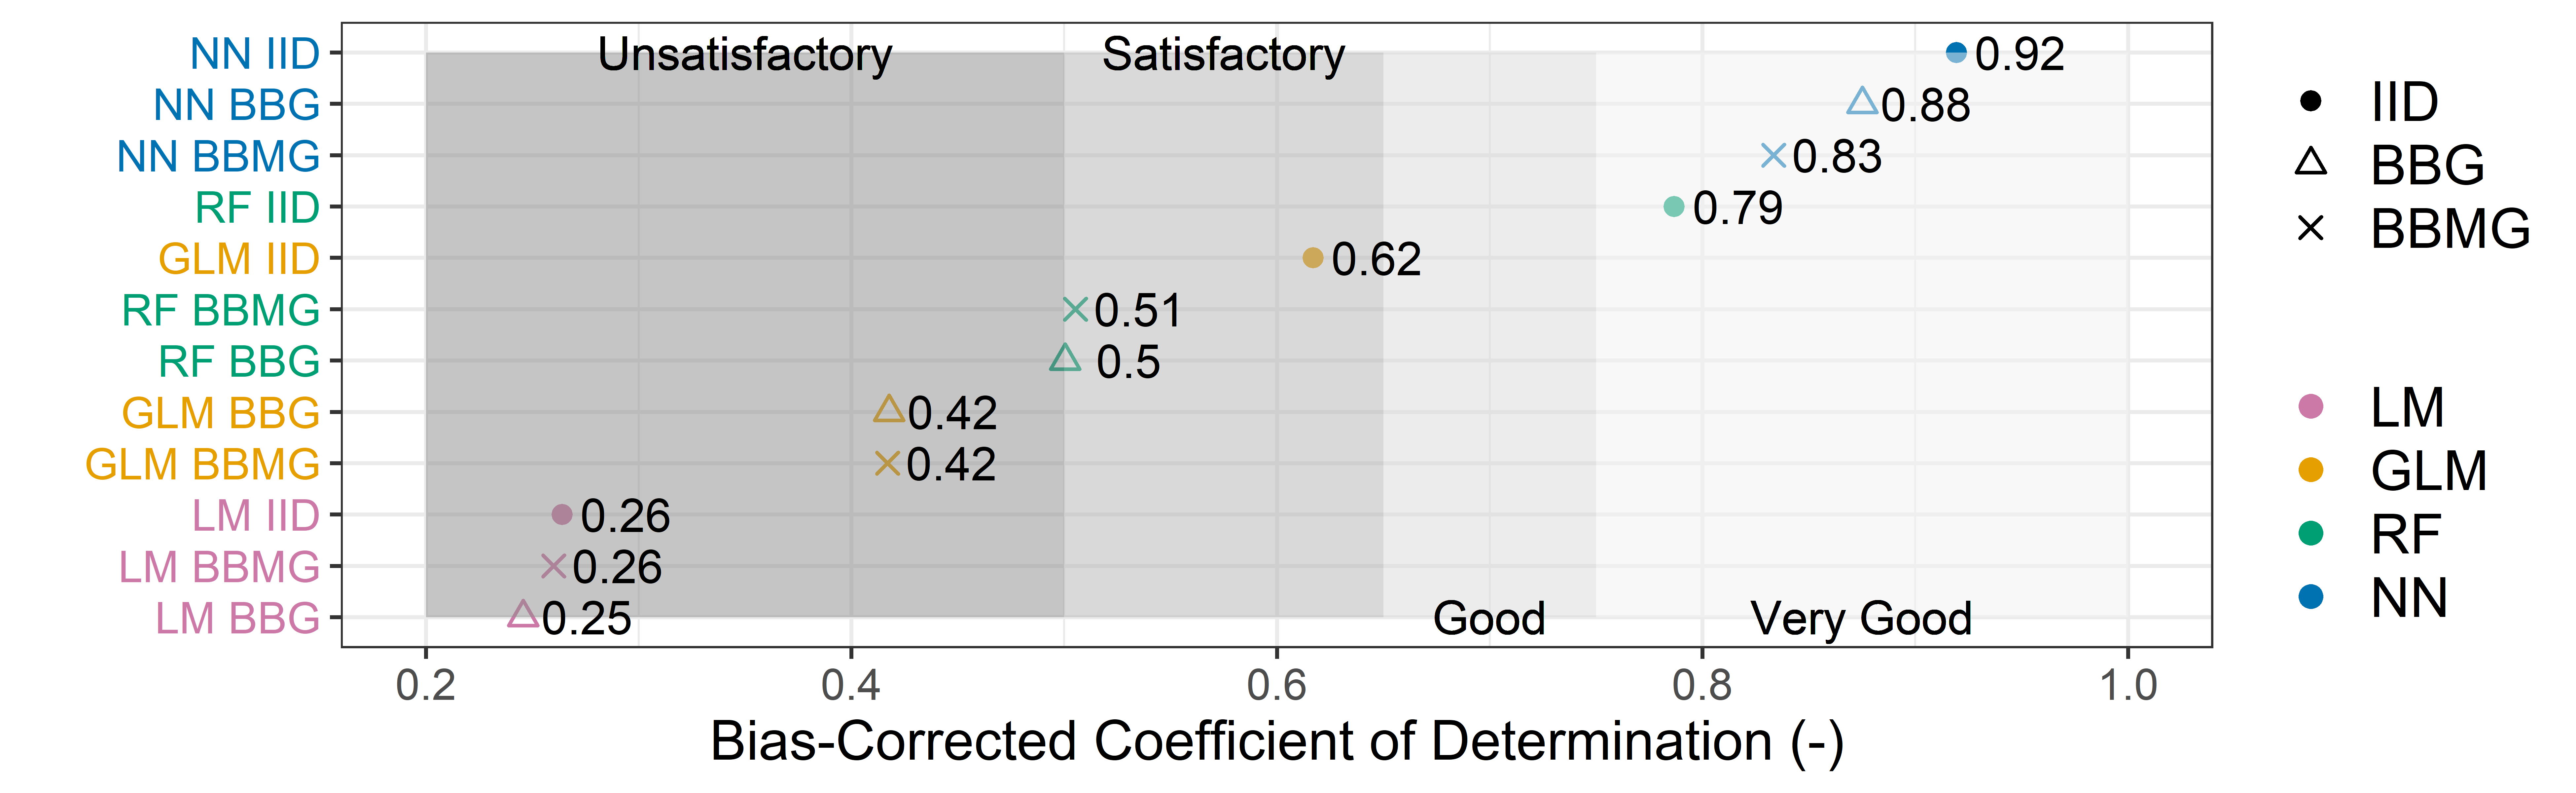
\includegraphics[width=\textwidth, trim={0 0 0 0}, clip=true]{plots/rplot41_gof_bR2_bs.png}
  		\caption{The average bootstrapping test set error.}
  		\label{fig:bsmoderror}
	\end{subfigure}
	\caption[Model goodness-of-fit and average goodness-of-fit given by cross-validation and bootstrapping strategies.]{Model goodness-of-fit and average goodness-of-fit given by cross-validation and bootstrapping strategies. Generally, in the LM, GLM, and RF models, the test set error is lower the smaller the block size or fold size. However, the NN prefers the more appropriate LOGO cross-validation strategy.}
	\label{fig:cvbserrors}
\end{figure}

Figure \ref{fig:cvbserrors2} shows model goodness-of-fit given by cross-validation and bootstrapping. (a) LM and GLM models are not as sensitive to cross validation strategies as NN and especially RF models. (b) bR\textsuperscript{2} values obtained where each dot is a simulation, with 100 simulations depicted in each line. The IID method generally under estimates model error in all four model types. In the BBG method, RF shows the biggest spread (standard deviation=0.19, N=100) and NN the lowest spread (standard deviation=0.07, N=100). In general, the bootstrap methods show the spread (or reliability) of an estimate more than cross-validation, which is why bootstrapping methods have become more popular in statistics. 

\begin{figure}
	\centering
	\begin{subfigure}{\textwidth}
  		\centering
 		 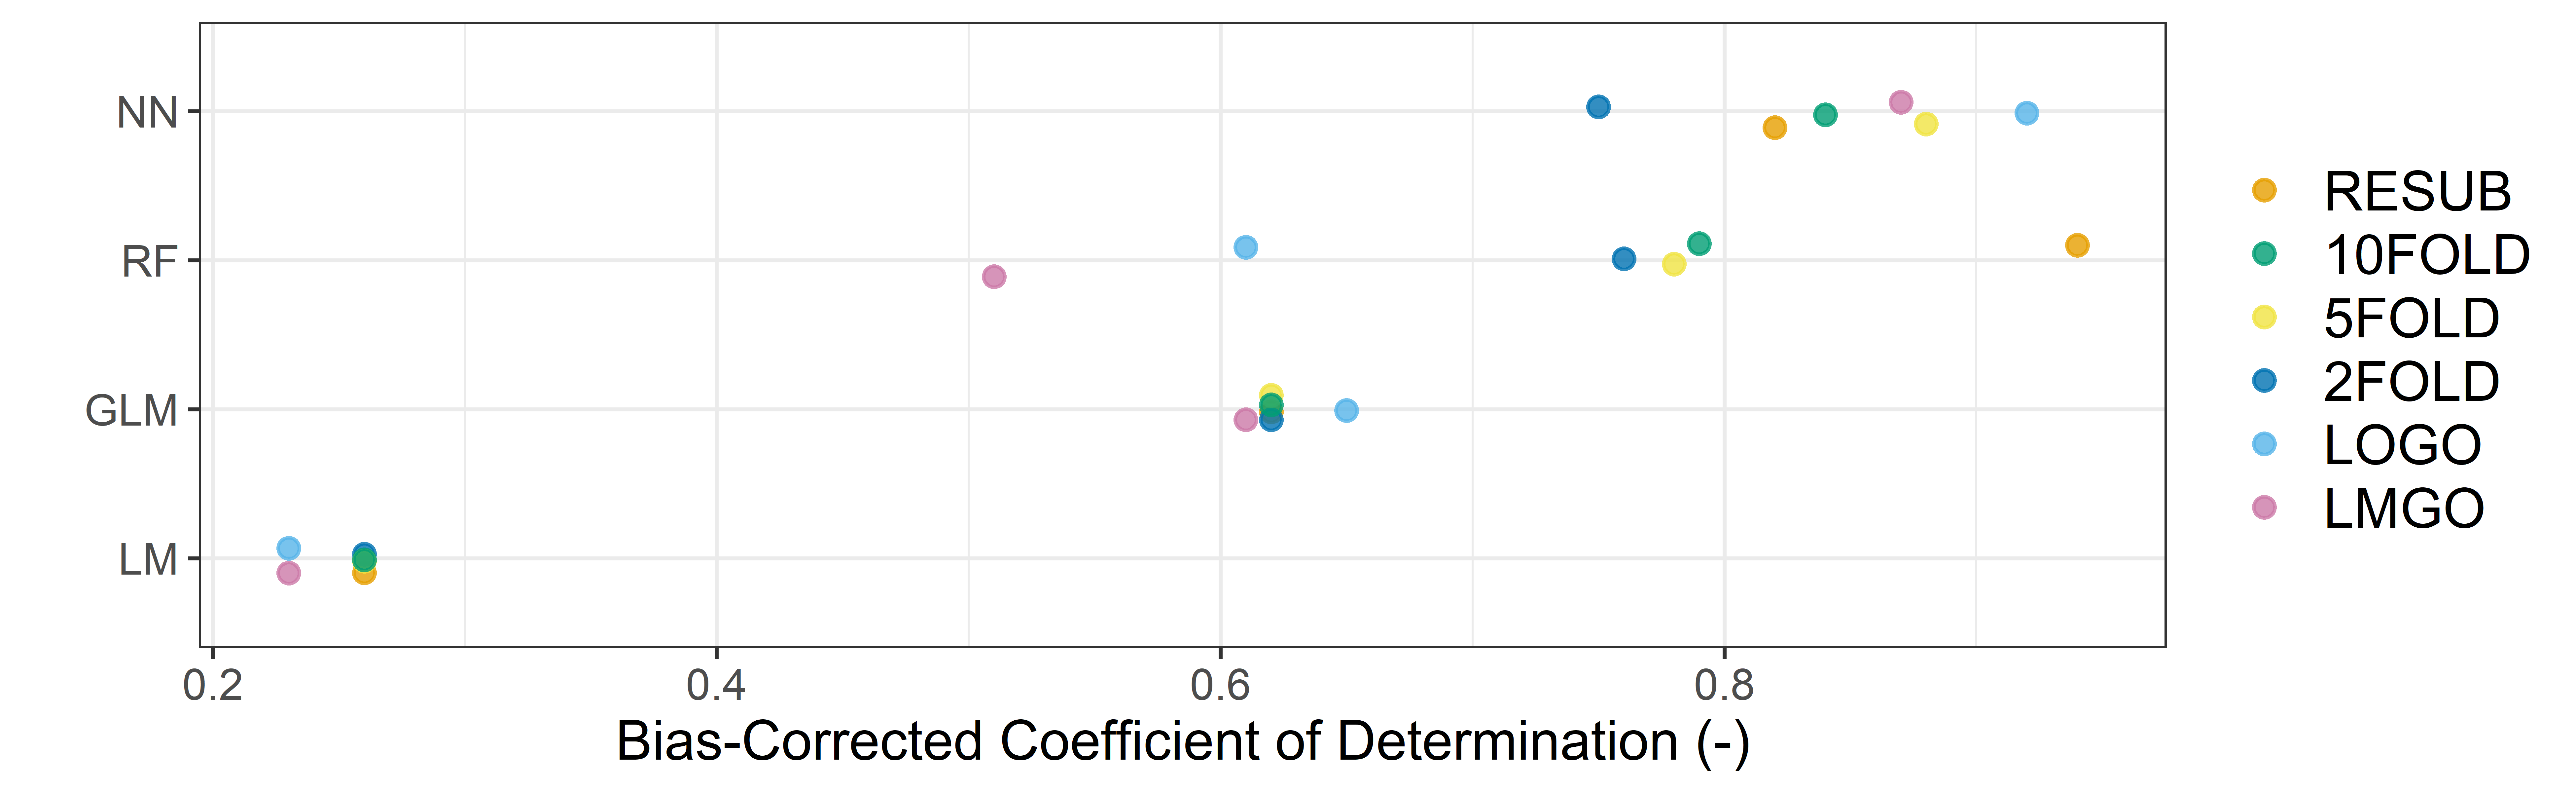
\includegraphics[width=\textwidth, trim={0 0 0 0}, clip=true]{plots/rplot42_gof_bR2.png}
  		\caption{The cross-validation test set error.}
  		\label{fig:cvmoderror2}
	\end{subfigure} 
	\begin{subfigure}{\textwidth}
  		\centering
  		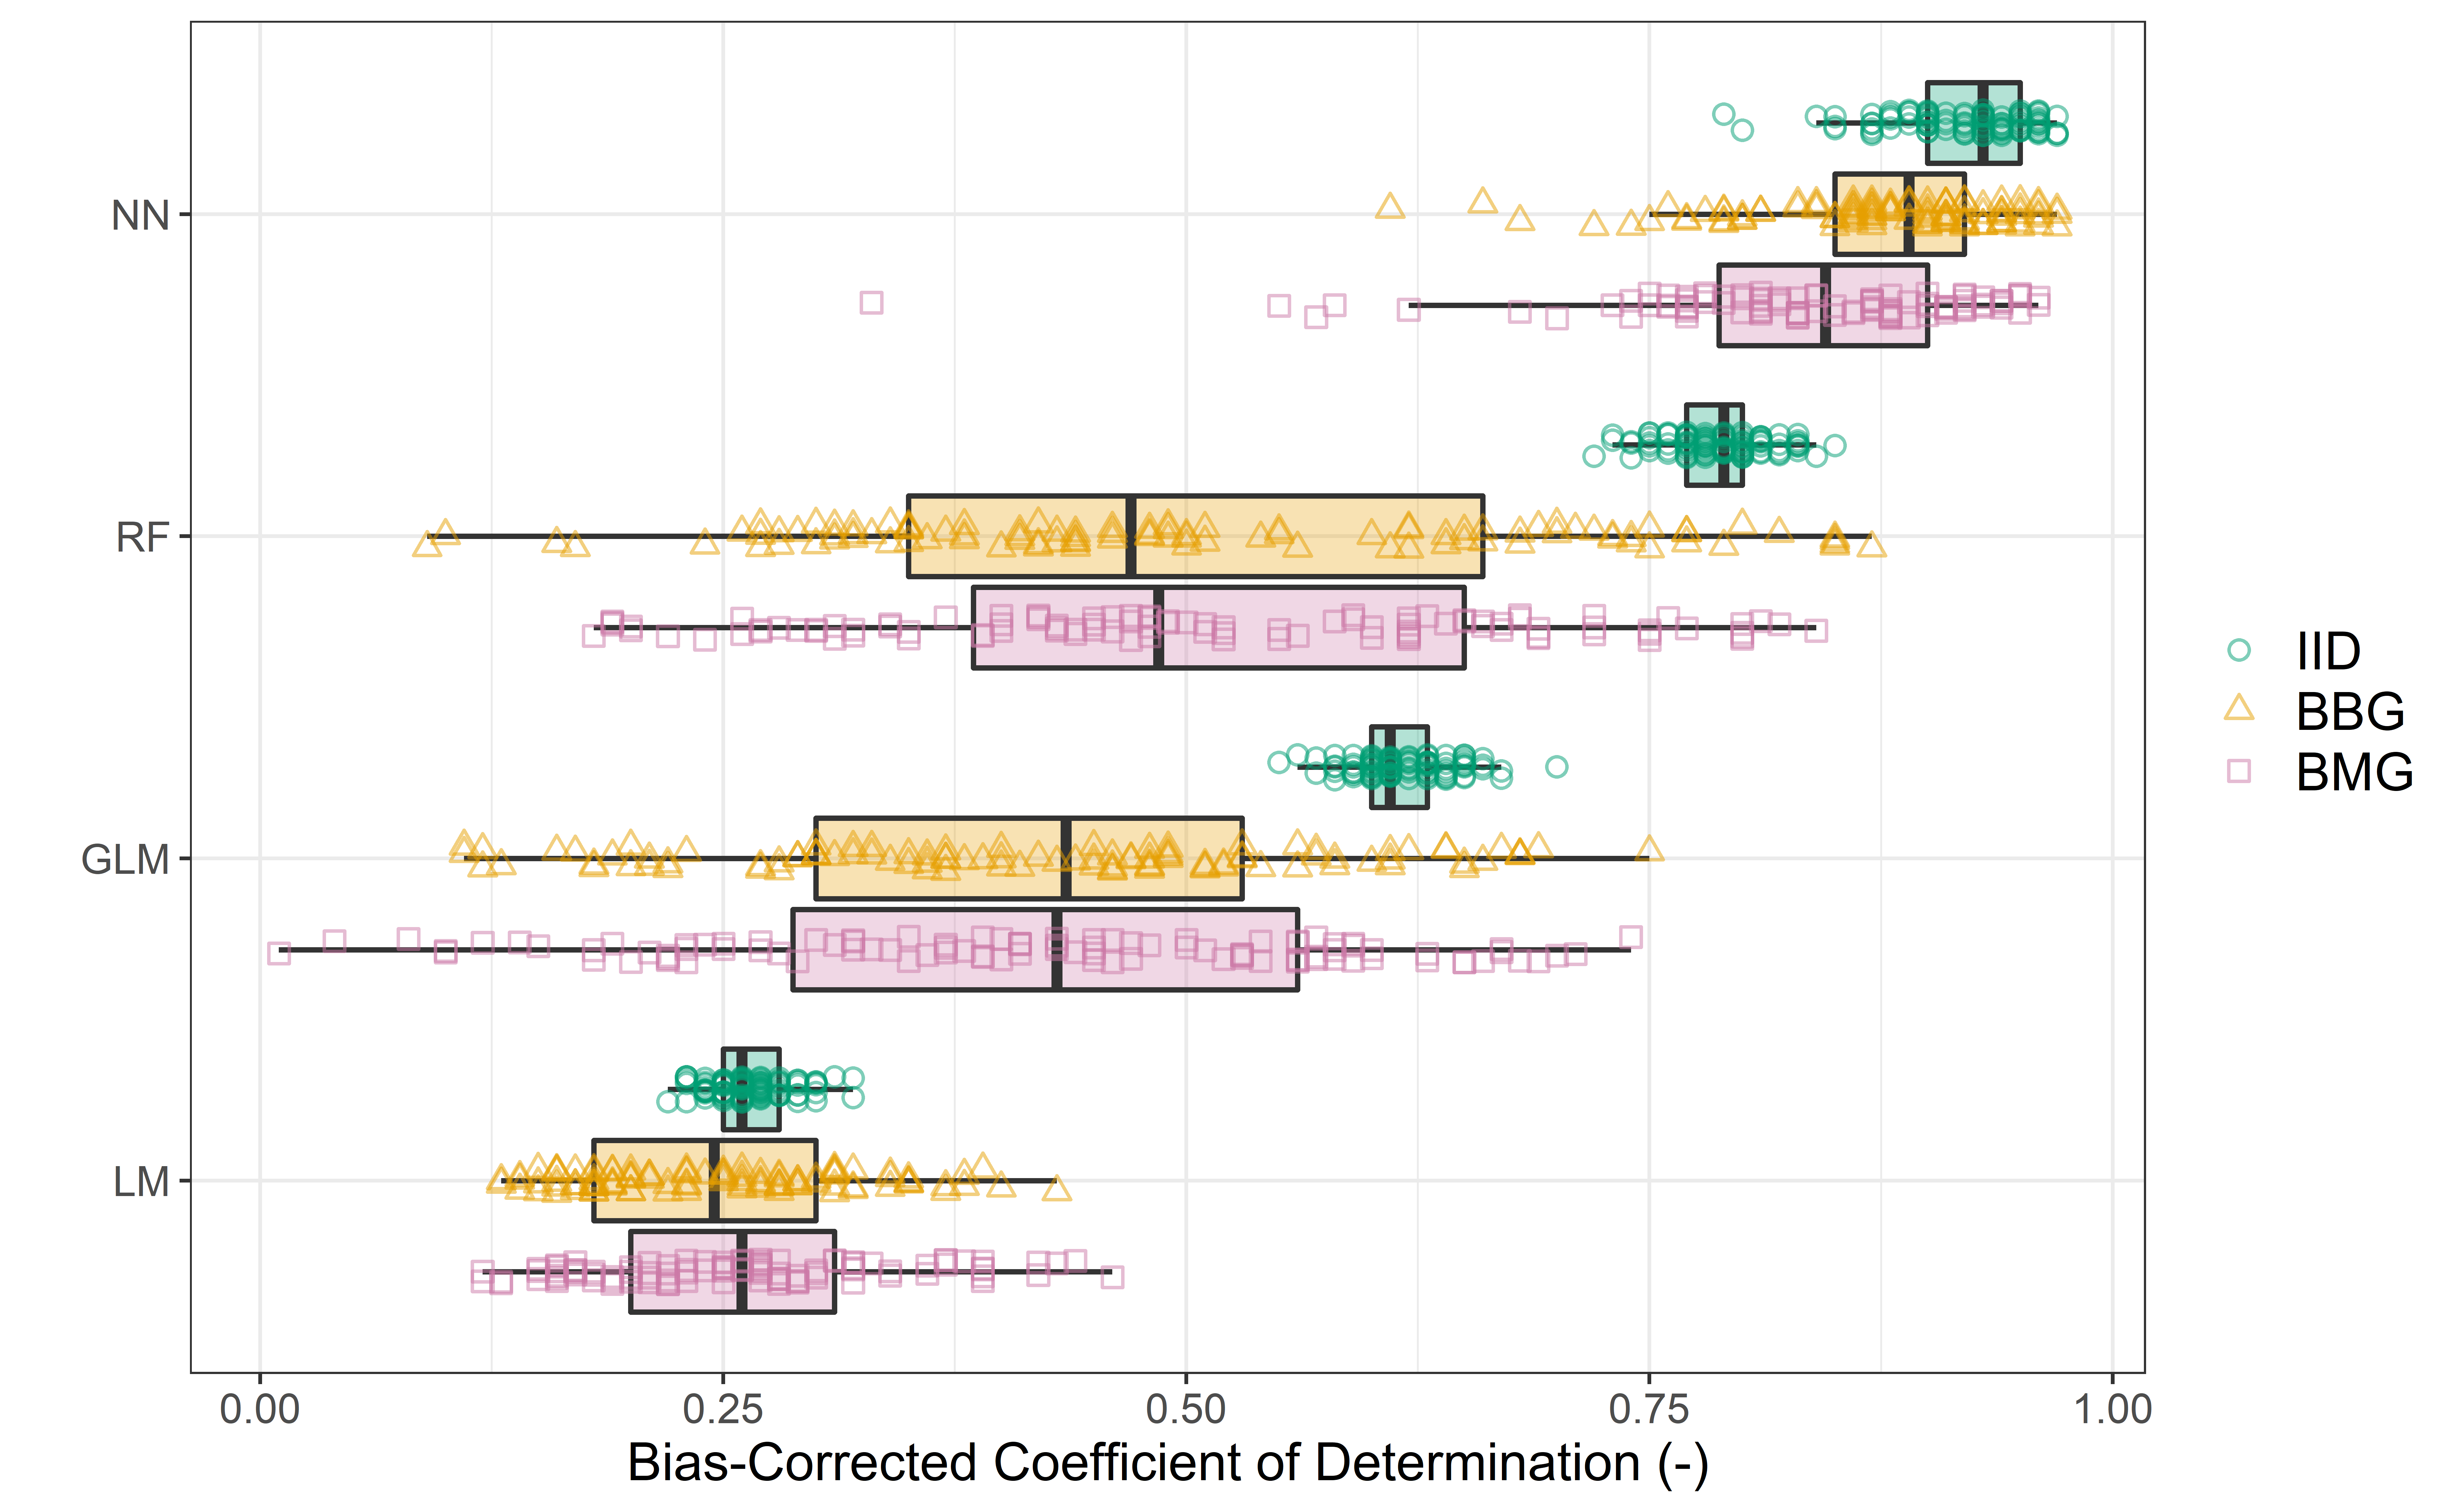
\includegraphics[width=\textwidth, trim={0 0 0 0}, clip=true]{plots/rplot42_gof_bR2_bs_boxplot.png}
  		\caption{The bootstrapping test set error.}
  		\label{fig:bsmoderror2}
	\end{subfigure}
	\caption[Model goodness-of-fit given by cross-validation and bootstrapping.]{Model goodness-of-fit given by cross-validation and bootstrapping (100 simulations per model per bootstrapping strategy). (a) The LM and GLM models are not as sensitive to cross validation strategies as NN and especially RF models. (b) The spread of the bR\textsuperscript{2} values obtained proving the value of having repeated experiments when estimating a model measure of fit.}
	\label{fig:cvbserrors2}
\end{figure}

Figure \ref{fig:obsprednn} shows the observed vs. predicted values for the NN model. It confirms the goodness-of-fit results; in LOGO cross-validation the points more closely fall along the line of best fit, $y=x$, with a slight tendency to underpredict (slope of the fitted line $\beta$=0.97). The lowest performance was with the LMGO method proving that grouping basins together can hide meaningful information from the model. In this method, the 67 basins are randomly grouped into 5 folds (block size=13 or 14 basins). Unsurprisingly, the performance degrades compared to the BBG method (block size=1 basin), where less information is held out from the model. 

\begin{figure}
	\centering
 	\includegraphics[trim={0 0 0 0}, clip=true]{plots/rplot43_obsvspred_all_nn.png}
  	\caption[NN observed vs. predicted for different cross-validation strategies.]{NN observed vs. predicted for different cross-validation strategies. NN's performance is not as sensitive to the cross-validation strategy and prefers the more appropriate LOGO method.}
  	\label{fig:obsprednn}
\end{figure}

Figure \ref{fig:obsprednnbs} shows that the goodness-of-fit obtained by bootstrapping decreases when switching to a blocking method, and the reliability in such measures decreases (standard deviation of bR\textsuperscript{2}=0.10 in BBMG vs. 0.03 in IID). Increasing block size decreases mean goodness-of-fit slightly (bR\textsuperscript{2}=0.88 in BBG vs. 0.83 in BBMG) and decreases the reliability of this estimate (standard deviation of bR\textsuperscript{2}=0.07 in BBG vs. 0.10 in BBMG). This is evident in the increase in spread and slight funnel shape (i.e., heteroscedasticity) of the plots as block sizes increase; withholding more information with bigger block sizes proves especially detrimental for accurately predicting lower flows. The data in the bootstrapping strategies somewhat confusingly have more variability and higher R\textsuperscript{2} as compared to the cross-validation strategies. The higher R\textsuperscript{2} is due to more data points being closer to the 1:1 line that are being plotted on top of one another. 


\begin{figure}
	\centering
 	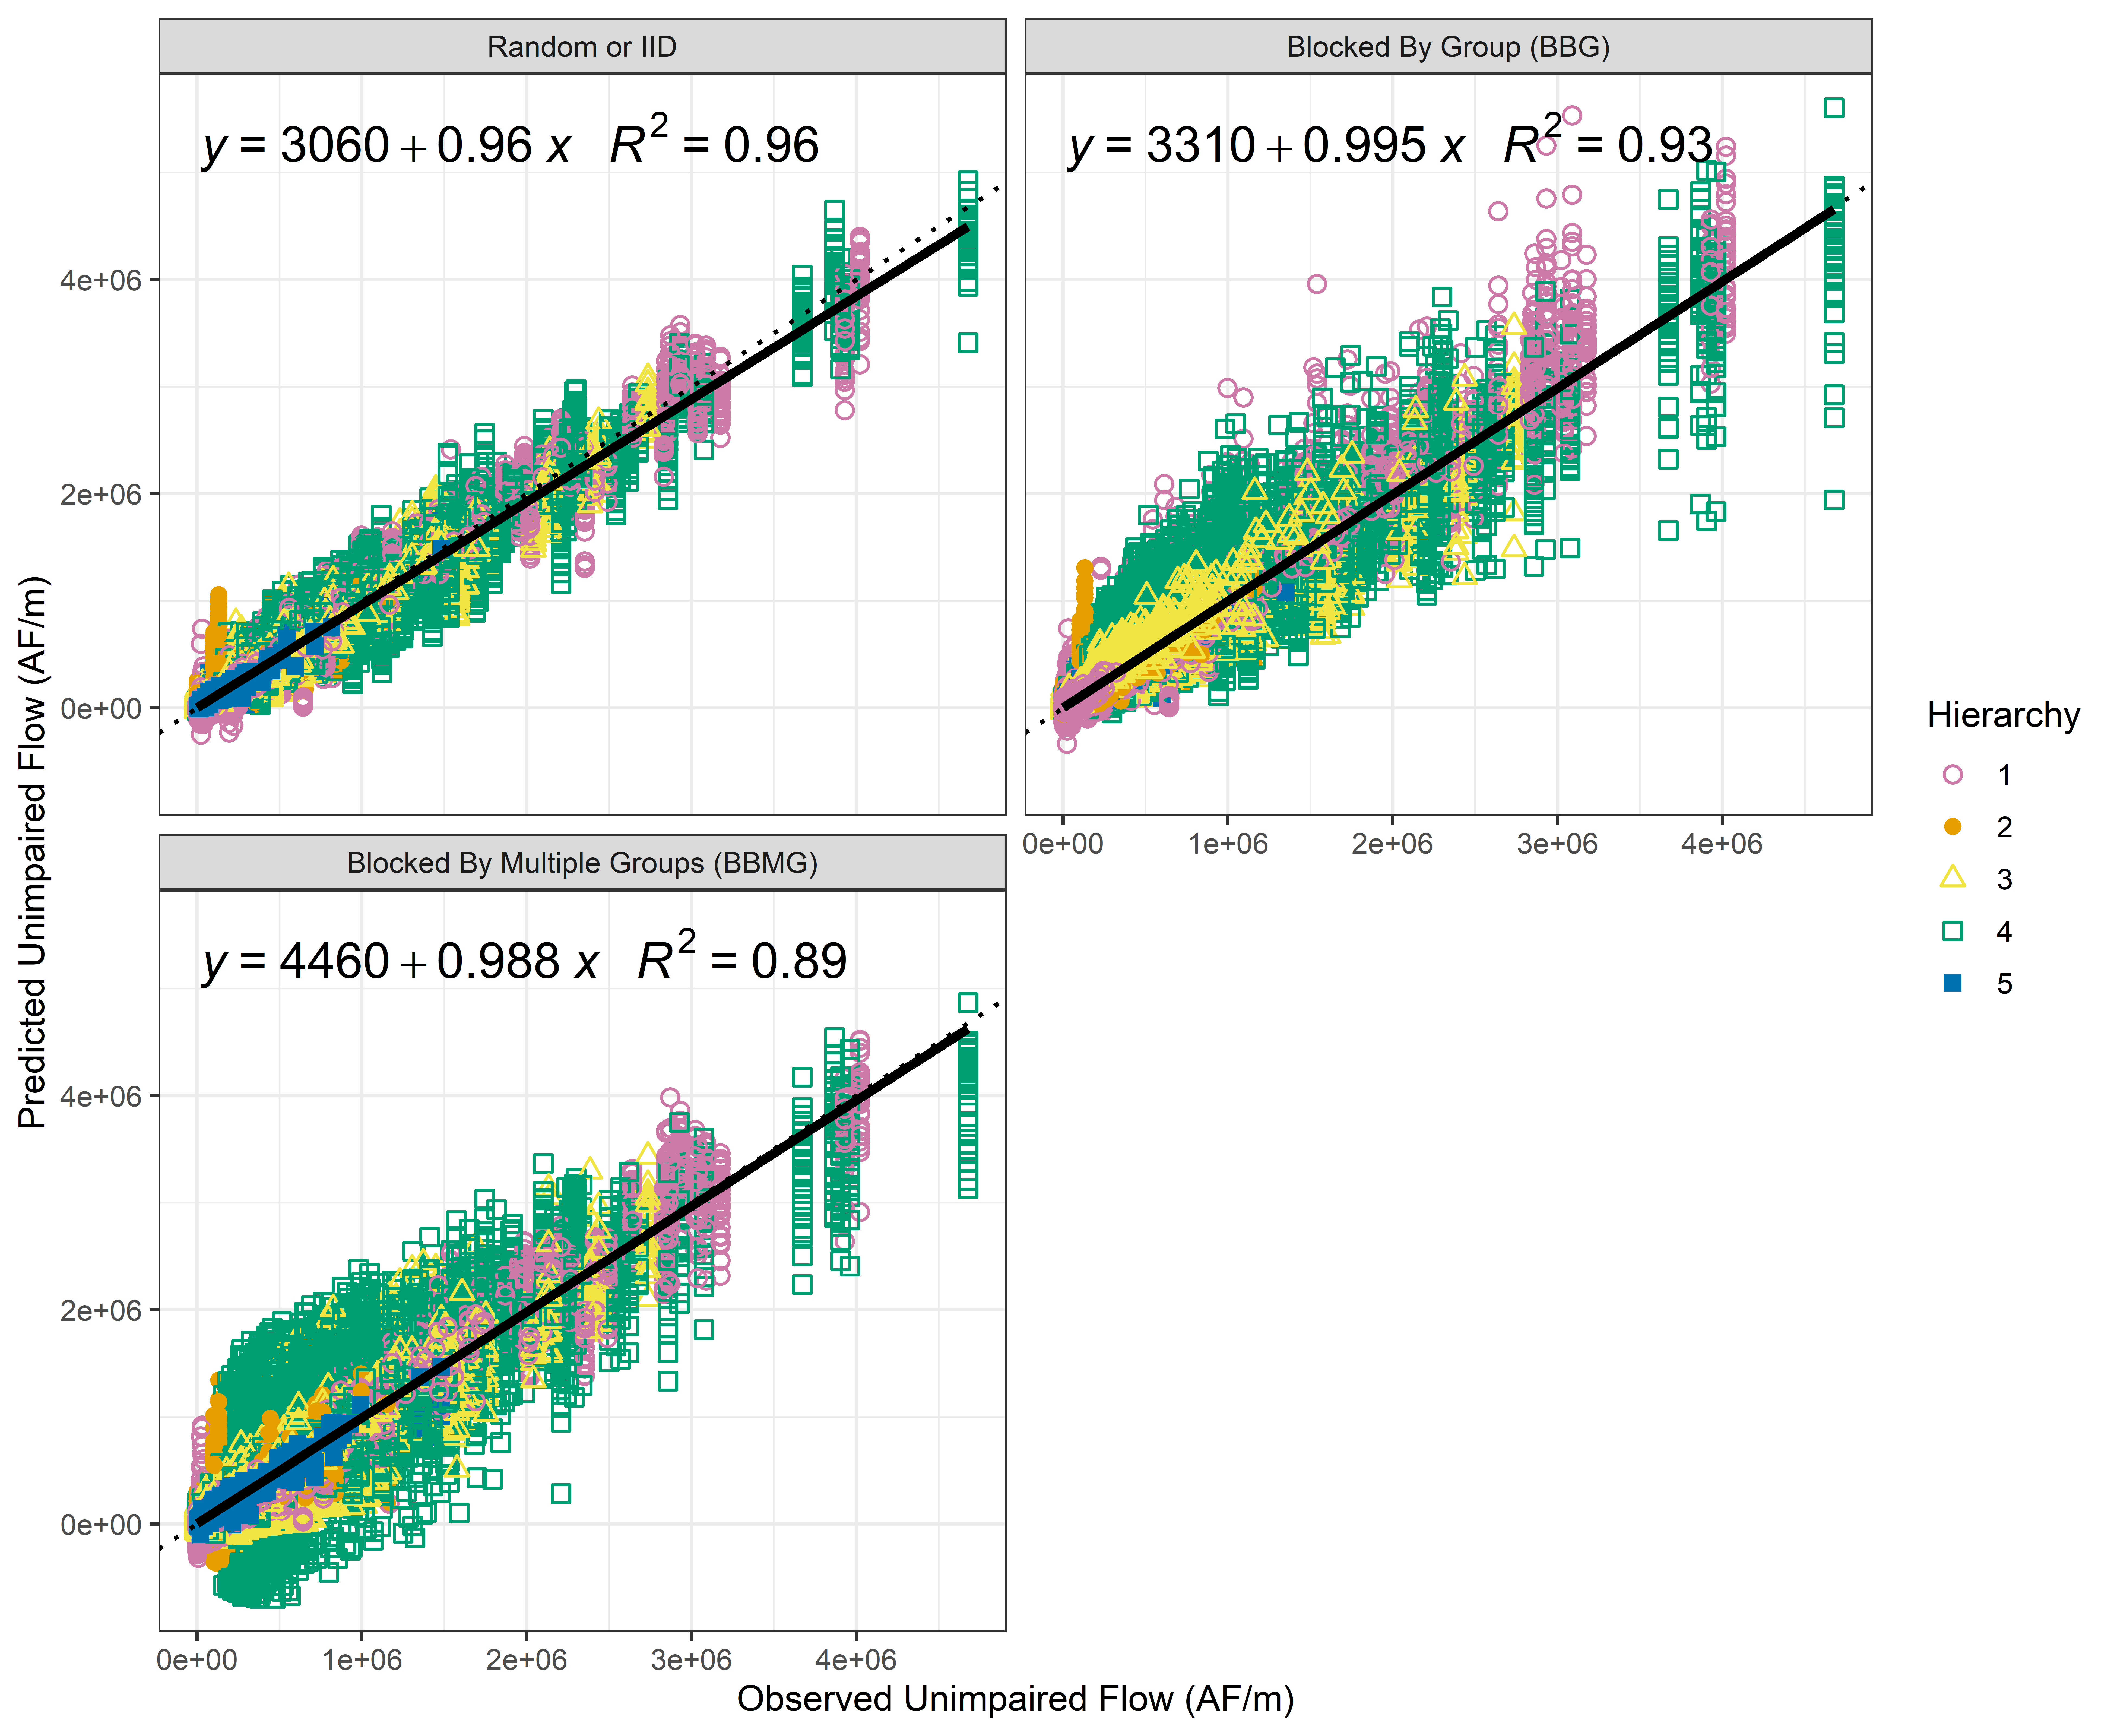
\includegraphics[trim={0 0 0 0}, clip=true]{plots/rplot44_obsvspred_bs_all_nn.png}
  	\caption[NN observed vs. predicted for different bootstrapping strategies.]{NN observed vs. predicted for different bootstrapping strategies (No. of simulations=100). As block sizes increase, the spread increases especially for low flows; withholding more information with bigger block sizes proves especially detrimental for accurately predicting lower flows.}
  	\label{fig:obsprednnbs}
\end{figure}

Figure \ref{fig:modelscvdensity} shows the density of predicted vs. observed unimpaired flows for cross-validation resampling. All models have a tendency to predict to the mean due to MSE being the loss function of choice. GLM, RF, and NN more accurately predict the frequency of ``floods'' (i.e. the right side tail). All models, except for the RESUB, 10 FOLD and 5 FOLD in the RF, fail to predict the frequency of ``droughts'' (i.e. the left side tail). As block sizes increase in the RF, the harder it becomes for the RF to predict droughts, much like other models. LM shows very little sensitivity to the cross-validation resampling method. GLM has a slight increase in low flow densities due to the Tweedie distribution (a semi-continuous function) defining variance in the $y$ values. Also, blocking strategies (i.e., LOGO and LMGO) have a slight improvement in predicting floods. In the RF, blocking strategies (i.e., LOGO and LMGO) more closely follow each other than the non-blocked methods, with the resubstitution method being closest to observed values. The LOGO and LMGO methods predict more floods compared to other non-blocked methods. In the NN, all methods except for the random two fold method follow each other, indicating that the 1/2 fold size, significantly affects the model. The fact that large folds or blocking itself produces higher flood densities may be due to the fact that in a model built with less data, the bigger flood values have more leverage in producing a flood sensitive model. 

\begin{figure}
  	\centering
 	\includegraphics[width=\textwidth, trim={0 0 0 0}, clip=true]{plots/rplot47_density_all.png}
	\caption[Cross-validation prediction density on a log transformed x axis.]{Cross-validation prediction density on a log transformed x axis. All models have a tendency to predict to the mean due to MSE being the loss function of choice. GLM, RF, and NN more accurately predict the frequency of ``floods'' (i.e. the right side tail). LM shows very little sensitivity to the cross-validation resampling method. GLM has a slight increase in low flow densities due to the Tweedie distribution (a semi-continuous function) defining variance in the $y$ values. Also, blocking strategies (i.e., LOGO and LMGO) have a slight improvement in predicting floods. In the RF, blocking strategies (i.e., LOGO and LMGO) more closely follow each other than the non-blocked methods, with the resubstitution method being closest to observed values. The LOGO and LMGO methods predict more floods compared to other non-blocked methods.}
	\label{fig:modelscvdensity}
\end{figure}

Figure \ref{fig:modelscvdensity_bs} shows the density of predicted vs. observed unimpaired flows for bootstrapped resampling. The observed value densities are also depicted and are slightly different from one another because in bootstrapping the dataset gets resampled. The densities here, much like with the cross-validation methods, show a regression to the mean due to MSE being the loss function of choice. In the LM, bootstrapping strategies are virtually indistinguishable. In the other models, the blocking strategies (i.e., BBG and BBMG) follow each other more closely than the IID. Just as in cross-validation, blocking produces higher flood densities.

\begin{figure}
  	\centering
 	\includegraphics[trim={0 0 0 0}, clip=true]{plots/rplot412_density_bs_all.png}
	\caption[Bootstrapping prediction density on a log transformed x axis.]{Bootstrapping prediction density on a log transformed x axis. In the LM, bootstrapping strategies are virtually indistinguishable. In the other models, the blocking strategies (i.e., BBG and BBMG) follow each other more closely than the IID, a non-blocking resampling method. Just as in cross-validation, blocking produces higher flood densities.}
	\label{fig:modelscvdensity_bs}
\end{figure}

% consider plotting and adding in residual densities here (?)
%
% I took these out because they don't add much to the discussion. Maybe add it to an appendix. 
%Figures \ref{fig:modelbr2dotchart} and \ref{fig:modelbr2dotchart_bs} show the bR\textsuperscript{2} and mean bR\textsuperscript{2} values disaggregated for each basin respectively. Generally, for all basins, in cross-validation, the LOGO method falls between LMGO and other methods. In bootstrapping, the IID over estimates and the BBMG under estimates goodness-of-fit, which confirms results from the aggregated plots mentioned before. The groupings based on hierarchies (numbers on the right side) show that generally the lower a basin is in the network the better it performs, especially in the NN. 
%
%\begin{figure}
%	\centering
%	\begin{subfigure}{\textwidth}
%  		\centering
% 		 \includegraphics[trim={0 0 0 0}, clip=true]{plots/rplot416_lm_bR2dotchart_comp.png}
%  		\caption{LM}
%  		\label{fig:lmbr2dotchart}
%	\end{subfigure}
%\end{figure}
%\begin{figure}\ContinuedFloat
%	\begin{subfigure}{\textwidth}
%  		\centering
%  		\includegraphics[trim={0 0 0 0}, clip=true]{plots/rplot416_glm_bR2dotchart_comp.png}
%  		\caption{GLM}
%  		\label{fig:glmbr2dotchart}
%	\end{subfigure}
%\end{figure}
%\begin{figure}\ContinuedFloat
%	\begin{subfigure}{\textwidth}
%  		\centering
%  		\includegraphics[trim={0 0 0 0}, clip=true]{plots/rplot416_rf_bR2dotchart_comp.png}
%  		\caption{RF}
%  		\label{fig:rfbr2dotchart}
%	\end{subfigure}
%\end{figure}
%\begin{figure}\ContinuedFloat
%	\begin{subfigure}{\textwidth}
%  		\centering
%  		\includegraphics[trim={0 0 0 0}, clip=true]{plots/rplot416_nn_bR2dotchart_comp.png}
%  		\caption{NN}
%  		\label{fig:nnbr2dotchart}
%	\end{subfigure}
%	\caption{The bR\textsuperscript{2} disaggregated by basin for cross-validation strategies.}
%	\label{fig:modelbr2dotchart}
%\end{figure}
%
%\begin{figure}
%	\centering
%	\begin{subfigure}{\textwidth}
%  		\centering
% 		 \includegraphics[trim={0 0 0 0}, clip=true]{plots/rplot417_lm_bR2dotchart_comp.png}
%  		\caption{LM}
%  		\label{fig:lmbr2dotchart_bs}
%	\end{subfigure}
%\end{figure}
%\begin{figure}\ContinuedFloat
%	\begin{subfigure}{\textwidth}
%  		\centering
%  		\includegraphics[trim={0 0 0 0}, clip=true]{plots/rplot417_glm_bR2dotchart_comp.png}
%  		\caption{GLM}
%  		\label{fig:glmbr2dotchart_bs}
%	\end{subfigure}
%\end{figure}
%\begin{figure}\ContinuedFloat
%	\begin{subfigure}{\textwidth}
%  		\centering
%  		\includegraphics[trim={0 0 0 0}, clip=true]{plots/rplot417_rf_bR2dotchart_comp.png}
%  		\caption{RF}
%  		\label{fig:rfbr2dotchart_bs}
%	\end{subfigure}
%\end{figure}
%\begin{figure}\ContinuedFloat
%	\begin{subfigure}{\textwidth}
%  		\centering
%  		\includegraphics[trim={0 0 0 0}, clip=true]{plots/rplot417_nn_bR2dotchart_comp.png}
%  		\caption{NN}
%  		\label{fig:nnbr2dotchart_bs}
%	\end{subfigure}
%	\caption{The bR\textsuperscript{2} disaggregated by basin for bootstrapping strategies.}
%	\label{fig:modelbr2dotchart_bs}
%\end{figure}

%-----------------------------------------------
\subsection{Spatial Distribution of Error}
Figures \ref{fig:modelcvgif} and \ref{fig:modelbsgif} show goodness-of-fit results spatially. In all models there is a ridge of basins (lower Sierra Nevada basins) that generally have better fit. These basins have larger flows and the models trying to predict these values are more accurate at the expense of poorly predicting lower flows seen predominantly in headwater basins. In all model types, generally, performance declines as fold/block sizes increase. 

\begin{figure}
	\centering
	\begin{subfigure}{0.5\textwidth}
		\centering
		\begin{frame}{}
        		\animategraphics[loop,controls]{1}{plots/ch4_gif_br2map/lm/cv/br2map-}{1}{6}
		\end{frame}
  		\caption{LM}
  		\label{fig:lmcvgif}
	\end{subfigure}%
	\begin{subfigure}{0.5\textwidth}
  		\centering
		\begin{frame}{}
        		\animategraphics[loop,controls]{1}{plots/ch4_gif_br2map/glm/cv/br2map-}{1}{6}
		\end{frame}
  		\caption{GLM}
  		\label{fig:glmcvgif}
	\end{subfigure}
	\hfill
	\begin{subfigure}{0.5\textwidth}
  		\centering
		\begin{frame}{}
        		\animategraphics[loop,controls]{1}{plots/ch4_gif_br2map/rf/cv/br2map-}{1}{6}
		\end{frame}
  		\caption{RF}
  		\label{fig:rfcvgif}
	\end{subfigure}%
	\begin{subfigure}{0.5\textwidth}
  		\centering
		\begin{frame}{}
        		\animategraphics[loop,controls]{1}{plots/ch4_gif_br2map/nn/cv/br2map-}{1}{6}
		\end{frame}
  		\caption{NN}
  		\label{fig:nncvgif}
	\end{subfigure}
	\hfill
	\caption[The spatial distribution of the model-measure-of fit given by the bR\textsuperscript{2} for cross-validation strategies.]{The spatial distribution of the model-measure-of fit given by the bR\textsuperscript{2} for cross-validation strategies. In all model types, generally, performance declines as fold sizes increase. 
}
	\label{fig:modelcvgif}
\end{figure}


\begin{figure}
	\centering
	\begin{subfigure}{0.5\textwidth}
		\centering
		\begin{frame}{}
        		\animategraphics[loop,controls]{1}{plots/ch4_gif_br2map/lm/bs/br2map-}{1}{3}
		\end{frame}
  		\caption{LM}
  		\label{fig:lmbsgif}
	\end{subfigure}%
	\begin{subfigure}{0.5\textwidth}
  		\centering
		\begin{frame}{}
        		\animategraphics[loop,controls]{1}{plots/ch4_gif_br2map/glm/bs/br2map-}{1}{3}
		\end{frame}
  		\caption{GLM}
  		\label{fig:glmbsgif}
	\end{subfigure}
	\hfill
	\begin{subfigure}{0.5\textwidth}
  		\centering
		\begin{frame}{}
        		\animategraphics[loop,controls]{1}{plots/ch4_gif_br2map/rf/bs/br2map-}{1}{3}
		\end{frame}
  		\caption{RF}
  		\label{fig:rfbsgif}
	\end{subfigure}%
	\begin{subfigure}{0.5\textwidth}
  		\centering
		\begin{frame}{}
        		\animategraphics[loop,controls]{1}{plots/ch4_gif_br2map/nn/bs/br2map-}{1}{3}
		\end{frame}
  		\caption{NN}
  		\label{fig:nnbsgif}
	\end{subfigure}
	\hfill
	\caption[The spatial distribution of the model-measure-of fit given by the bR\textsuperscript{2} for bootstrapping strategies.]{The spatial distribution of the model-measure-of fit given by the bR\textsuperscript{2} for bootstrapping strategies. In all model types, generally, performance declines as block sizes increase. }
	\label{fig:modelbsgif}
\end{figure}
%-----------------------------------------------------------------------------------------------------------------------------------------------------------------------------------------------------
\section{Conclusion}
This chapter presented various blocking resampling techniques where the observations in a block are bonded together. The idea behind blocked resampling is simple: \textit{birds of a feather flock together}, or more accurately birds of a feather \textit{should} flock together (Figure \ref{fig:birds}). That is, if two observations are autocorrelated they should be both included in the bag, or training set, or both be out-of-bag, or in the test set. 

\begin{figure}
  	\centering
  	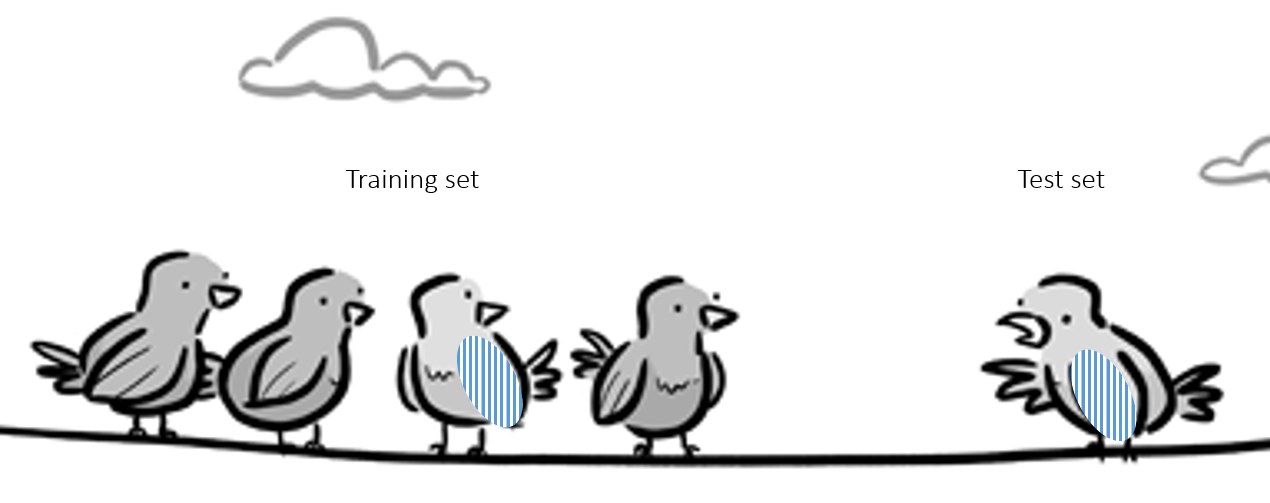
\includegraphics[width=0.5\textwidth, trim={0 0 0 0}, clip=true]{plots/ch4_birds.png}
  	\caption[The idea behind blocked resampling.]{The idea behind blocked resampling. Birds of a feather \textit{should} flock together.}
  	\label{fig:birds}
\end{figure}

These blocking methods show how much random ones underestimate model error. Models evaluated with random methods have artificially low errors due to the pseudo-replication from autocorrelation. This is not to say that, in hydrology, random resampling is never useful; a random test-train split is most appropriate for predicting flow for a sparsely incomplete gauge record. Blocked resampling in time is most appropriate for predicting or extrapolating streamflow in time for that location. One should not expect to use these resampling strategies and get the same predictive accuracy in a purely ungauged basin problem, where blocks are supposed to be designed across geographic space (or more accurately hierarchical structure). Results show that generally model performance estimates decline as block sizes increase. 

Some modeling methods are more sensitive to the resampling scheme than others. The LM performs poorly and is least sensitive. The RF is the most sensitive quite possibly due to the fact that it uses bootstrapping to construct a tree. The NN, performs well with all resampling strategies and surprisingly, performs better given the LOGO cross-validation strategy. The bootstrapping results also show how much variance there could be around a particular error estimate and the importance of the field moving away from cross-validation that gives one estimate of the error to bootstrapping that can give an estimate of the reliability of the error as well. Larger fold sizes and blocked strategies seem to favor predicting more floods, which could be due to the fact that fewer data available to the model gives more leverage to observations with a higher value (especially when using the MSE loss function).


%Finally, resampling for model error estimation should follow these steps: \\
%(1) Does the data show dependence structures? Access the degree of dependence. \\
%(2) Determine modeling objective: i) to complete a sparsely missing record? ii) to predict in time in the past iii) to predict in space in the past iv) to predict into the future. \\
%(3) Design the cross-validation strategy depending on the modeling objective and the dependence structures identified. \\
%(4) Make one model for each fold or each resample. \\
%(5) Determine the suitability and applicability of the model. \\
%(6) Make final predictions using a full model. 




